%!TEX program = xelatex
%%%%%%%%%%%%%%%%%%%%%%%这是导言部分的开始%%%%%%%%

%========= 导言部分声明文档的类型=================
\documentclass{article}

%=========导言部分可可以加载宏包=================
\usepackage{amsmath}                % 数学公式排版宏包
\usepackage{amssymb}                % 数学符号命令宏包
\usepackage{amsthm}                 % 数学定理宏包
\usepackage[UTF8]{ctex}             % 中文输入宏包
\usepackage[a4paper]{geometry}      % 页面设置宏包
\usepackage{setspace}               % 行间距宏包
\usepackage{graphicx}               % 图片宏包
\usepackage{listings}               % 代码宏包
\usepackage{color}					% 颜色宏包
\usepackage{xcolor}                 % 颜色处理宏包
\usepackage{float}                  % 浮动对象式样宏包
\usepackage{fontspec}
\usepackage{enumerate}				% 列举编号包

%=========页面设置==============================
\geometry{left=1cm,right=1cm,top=1cm,bottom=2cm}
\onehalfspacing
\setlength\parindent{0em}

%=========代码格式设置============================
\definecolor{dkgreen}{rgb}{0,0.6,0}
\definecolor{gray}{rgb}{0.5,0.5,0.5}
\definecolor{mauve}{rgb}{0.58,0,0.82}
% \setmonofont{Consolas}
\lstset{
	numbers = left, 	
	numberstyle = \color{gray}, 
	keywordstyle = \color{blue},
	commentstyle = \color{dkgreen}, 
	stringstyle = \color{mauve},
	basicstyle = \ttfamily,
	breaklines = true,
	frame = shadowbox, % 阴影效果
	rulesepcolor = \color{ red!20!green!20!blue!20} ,
	escapeinside = ``, % 英文分号中可写入中文
	xleftmargin = 2em,xrightmargin=2em, aboveskip=1em,
	framexleftmargin = 2em
} 

%=========导言部分可以定义标题信息===============
\title{组会报告}
\author{徐益}
\date{\today}
%%%%%%%%%%%%%%%%%%%%%%%这是导言部分的结束%%%%%%%%%

%%%%%%%%%%%%%%%%%%%%%%%这是正文部分的开始%%%%%%%%%
\begin{document}

%=========生成标题================================
\maketitle

%=========开始正文的输入==========================

%===========第一节=================
\section{工作内容} 
1. 编写多线程编码调制程序;

2. 编写并调试与MAC层的对接程序。

%===========第二节=================
\section{编写多线程编码调制程序}
\subsection{程序结构}
\begin{figure}[H]
	\centering
	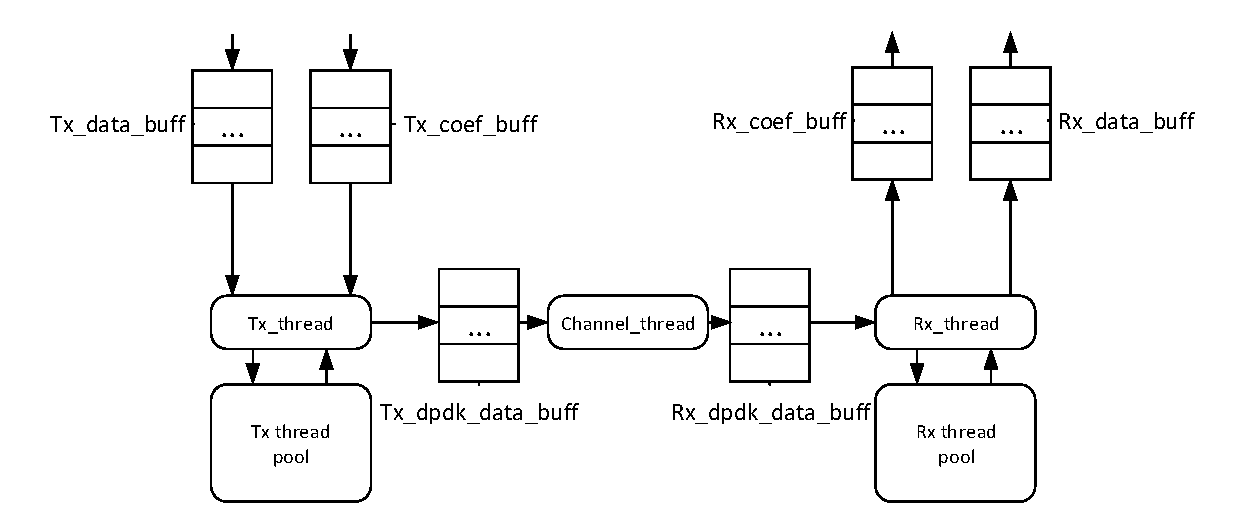
\includegraphics[width = \textwidth]{multi.pdf}
	\caption{多线程编码调制程序结构}
\end{figure}

\subsection{问题及解决情况}
\subsubsection{导频序列的三重指针难以向子线程传递}
已解决。改变导频序列结构为一维数组。
\subsubsection{发送端线程输出无法直接作为接收端线程输入}
已解决。增加信道线程。
\subsubsection{发送端时延过大}
\begin{figure}[H]
	\centering
	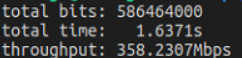
\includegraphics[width = .4\textwidth]{res.png}
	\caption{时延过大}
\end{figure}
待解决。对编码阶段进一步分割。

%===========第三节=================
\section{编写并调试与MAC层的对接程序}
\subsection{程序结构}
\begin{figure}[H]
	\centering
	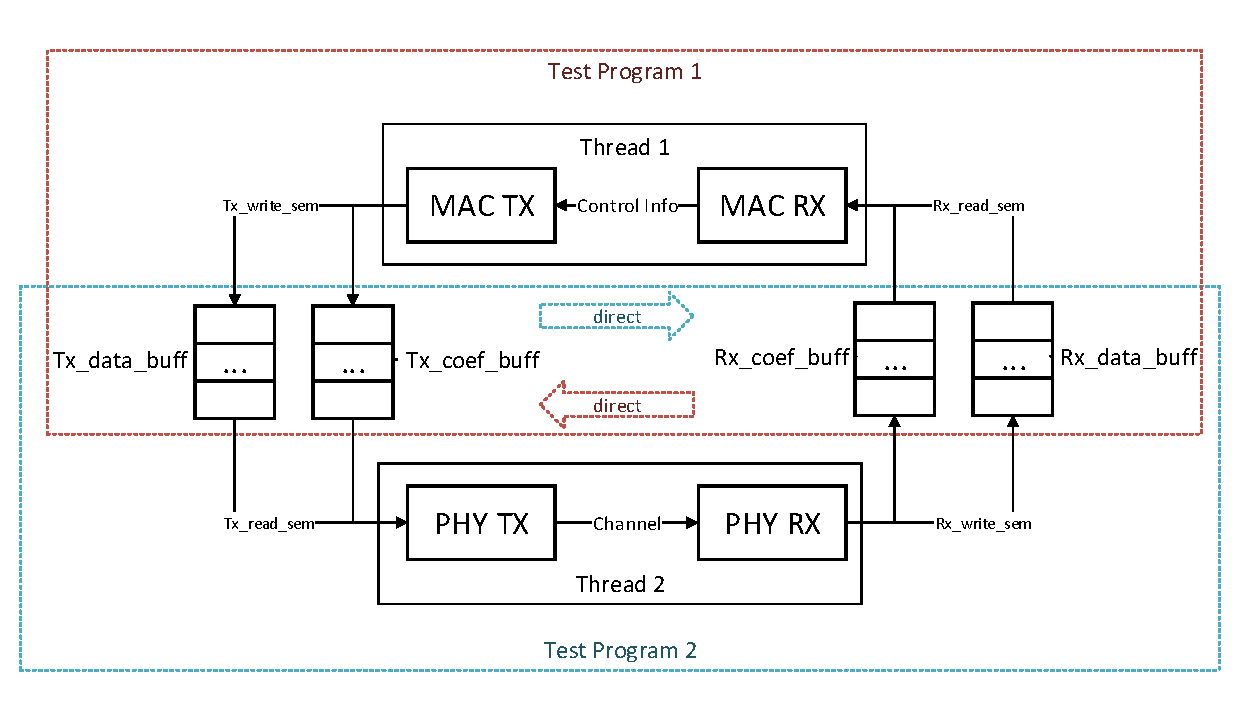
\includegraphics[width = \textwidth]{structure.pdf}
	\caption{与MAC层的对接程序结构}
\end{figure}
\subsection{当前问题}
在没有错报的情况下程序正常运行;\\
在有错包后的一段时间程序出现内存溢出。
\begin{figure}[H]
	\centering
	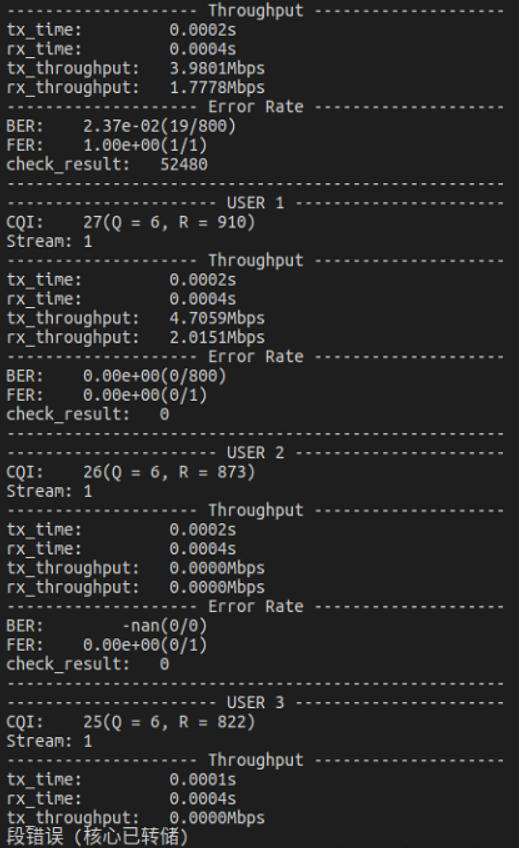
\includegraphics[width = .6\textwidth]{err.png}
	\caption{内存溢出}
\end{figure}

%===========第四节=================
% \section{编写多线程编码调制模块}
% \subsection{多线程结构}
% \begin{figure}[H]
% 	\centering
% 	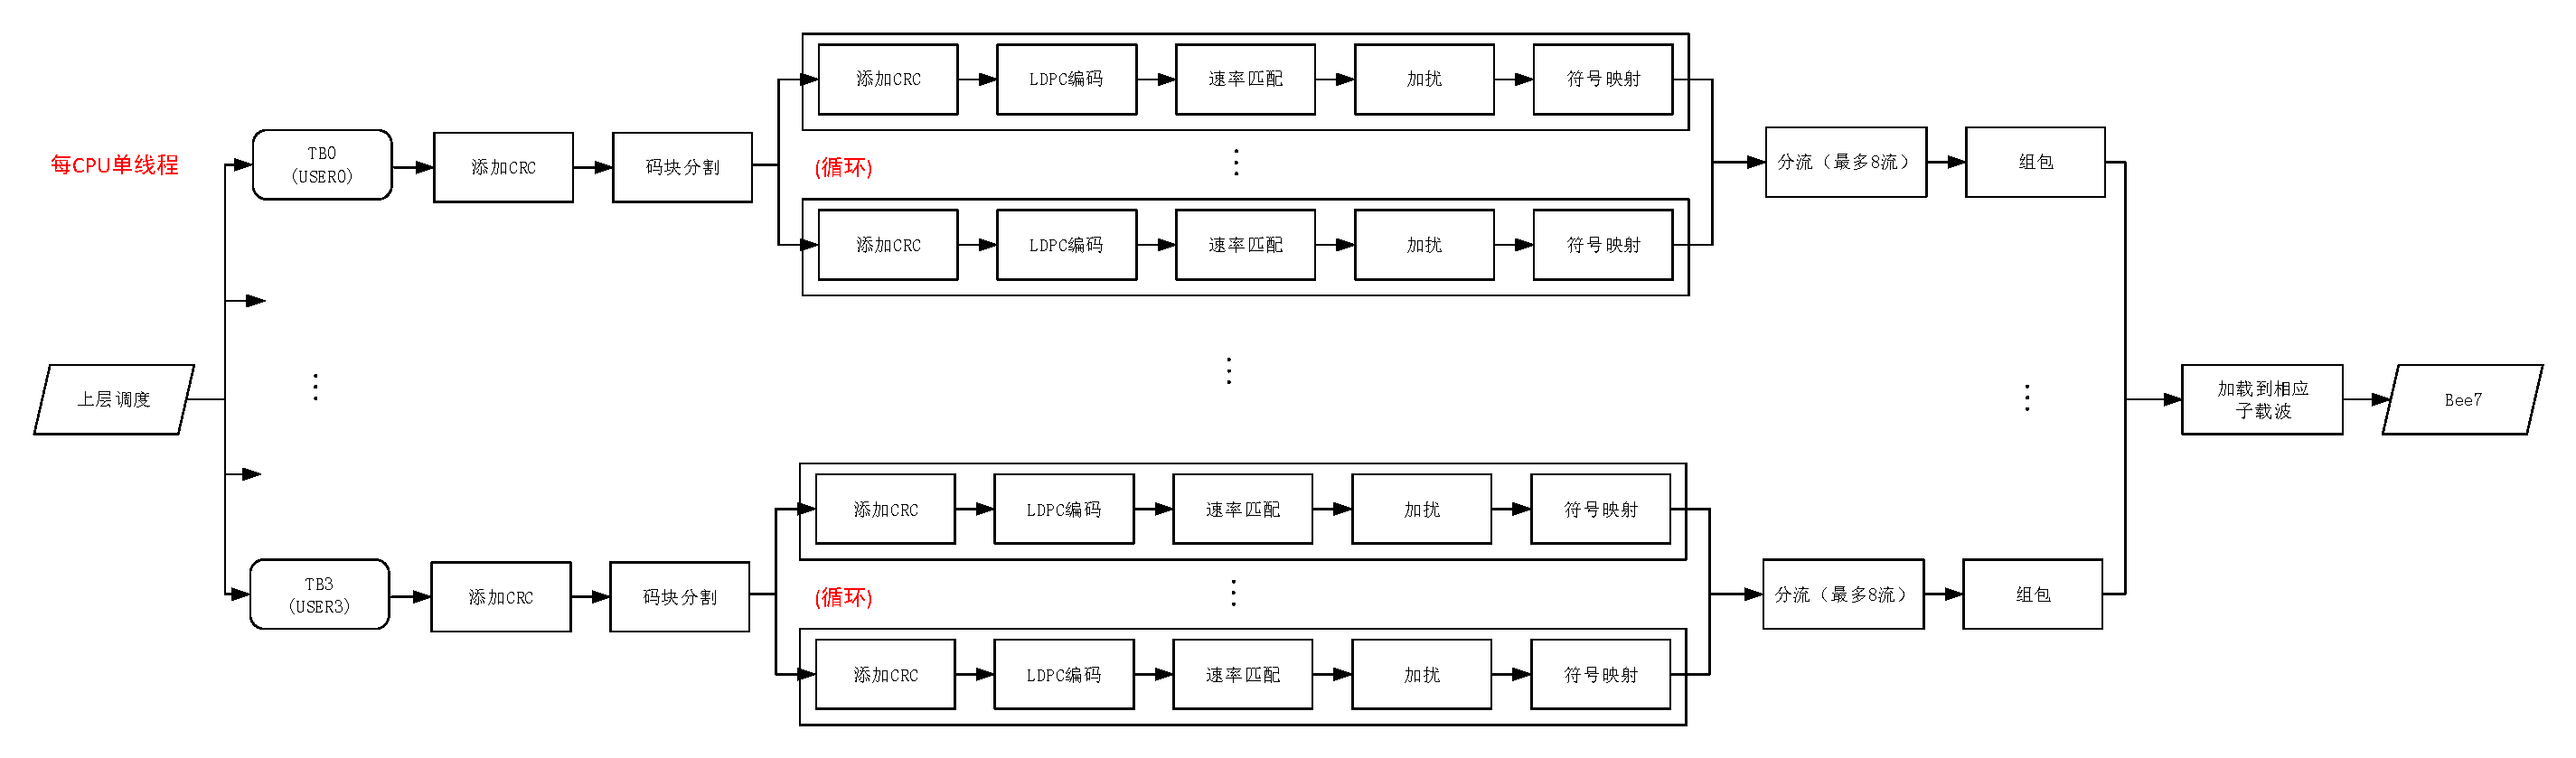
\includegraphics[width = \textwidth]{txstru.pdf}
% 	\caption{Tx结构}
% \end{figure}
% \begin{figure}[H]
% 	\centering
% 	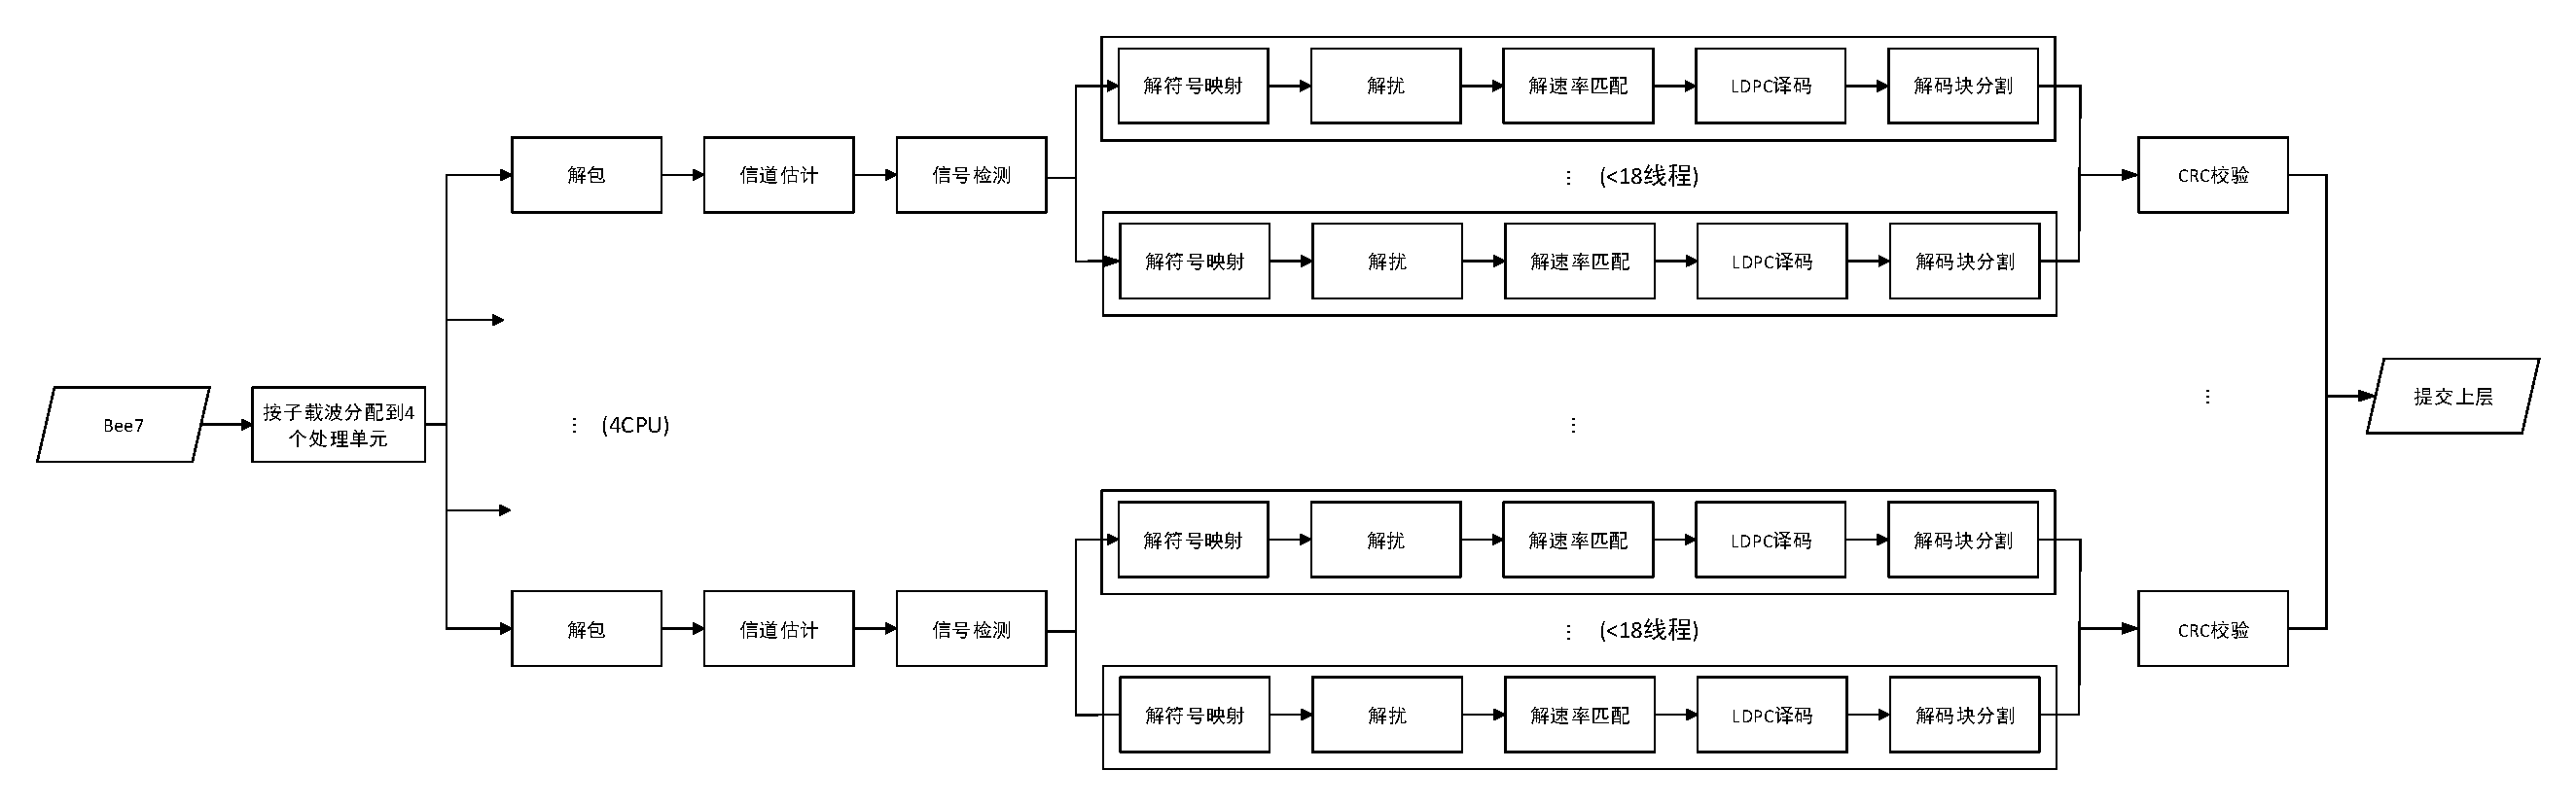
\includegraphics[width = \textwidth]{rxstru.pdf}
% 	\caption{Rx结构}
% \end{figure}
% \subsection{修改点}
% 1. 信号量传递由全局变量改为线程传参;\\
% 2. 轮巡式调度改为信号量调度; \\
% 3. 尝试简化线程阶段。

%===========第五节=================
% \section{有PRACH情况下的资源分配问题}
% \begin{figure}[H]
% 	\centering
% 	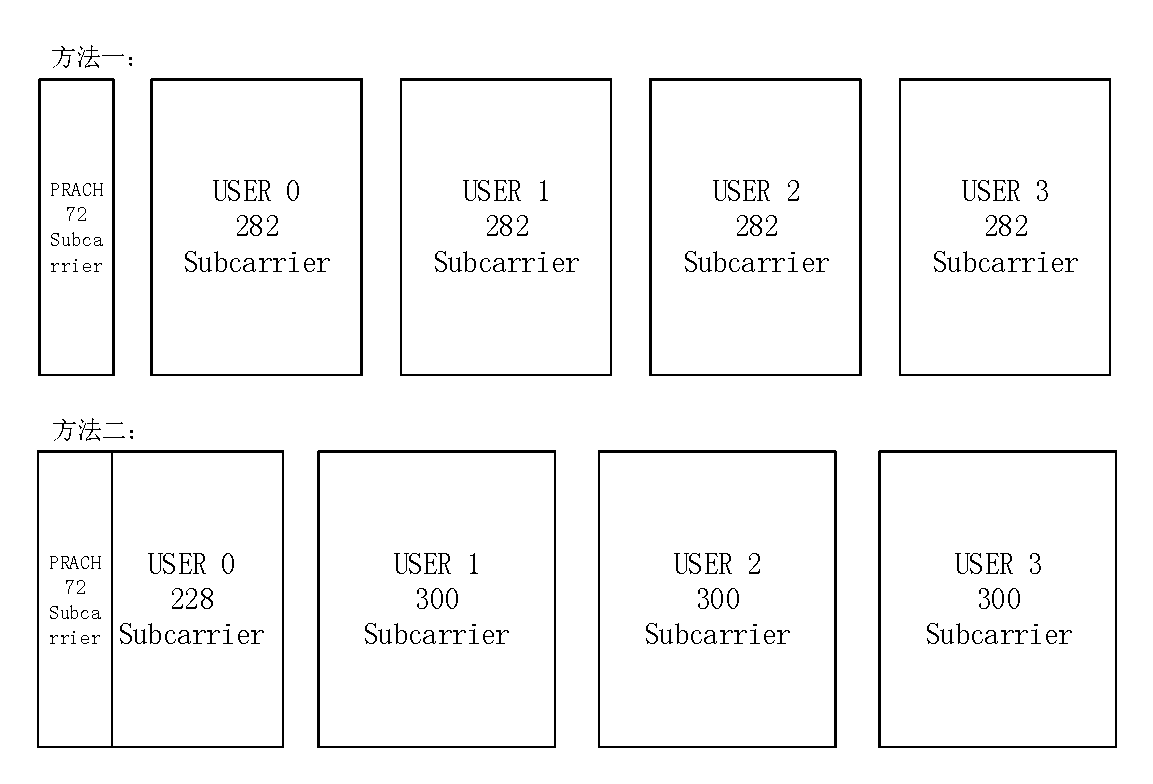
\includegraphics[width = \textwidth]{ques.pdf}
% 	\caption{两种方案}
% \end{figure}

%===========下周计划=================
% \section{下阶段计划}
% 1. 完善单线程系统(修复Bug)

\end{document}
%%%%%%%%%%%%%%%%%%%%%%%这是正文部分的结束%%%%%%%%%%%%